\documentclass[12pt]{article}
\usepackage[table]{xcolor}
\usepackage[shortlabels]{enumitem}
\usepackage{tabularx,xltabular}
\usepackage{graphicx}
\usepackage{hyperref}
\usepackage{verbatim}
\usepackage{geometry}
\usepackage{ulem}
\usepackage[official]{eurosym}
\usepackage{tikz}
\usetikzlibrary{arrows,backgrounds,calc,decorations.markings,patterns,3d}
\usepackage{pgfplots}
\pgfplotsset{compat = newest}
\usetikzlibrary{fit}
\newcommand\addvmargin[1]{
\usetikzlibrary{arrows}
\node[fit=(current bounding box),inner ysep=#1,inner xsep=0]{};}
\usepackage{cancel}
\usepackage{fontspec}
\usepackage{array}  
\geometry{a4paper, top=2cm, left=2cm, right=2cm, bottom=2cm, headsep=1cm}
\usepackage{tabu}
\usepackage{pst-node}
\usepackage{colortbl}
\usepackage{array}
\usepackage{german}
\setlength\parindent{0pt}
\newcolumntype{?}{!{\vrule width 1pt}}
\usepackage{makecell}
\renewcommand{\arraystretch}{2.5}
\usepackage{pbox}
\usepackage{amssymb}
\usepackage{amsmath}
\usepackage{booktabs}
\newcolumntype{L}[1]{>{\raggedright\let\newline\\\arraybackslash\hspace{0pt}}m{#1}}
\newcolumntype{C}[1]{>{\centering\let\newline\\\arraybackslash\hspace{0pt}}m{#1}}
\newcolumntype{R}[1]{>{\raggedleft\let\newline\\\arraybackslash\hspace{0pt}}m{#1}}
\begin{document}
\rightline{Datum: 08.06.2023}
\centerline{{\Large Tägliche Übungen}} 
\vspace{1cm}
\noindent \\


\begin{xltabular}{\textwidth}{|C{0.75cm}|X|C{0.75cm}|X|}
\arrayrulecolor{black}\hline
a)&$\begin{aligned}
 z=&7~ \rightarrow ~ 4 + 3 \cdot z=?
\end{aligned}$
&
b)&$\begin{aligned}
 x=&-7~ \rightarrow ~ x - 4=?
\end{aligned}$
\\\hline
c)&$\begin{aligned}
 a=&-12~ \rightarrow ~ 4 \cdot a + 2=?
\end{aligned}$
&
d)&$\begin{aligned}
 a=&8~ \rightarrow ~ 3 + a=?
\end{aligned}$
\\\hline
e)&$6\cdot a-17=19$
&
f)&$6\cdot b-19=41$
\\\hline
g)&$5\cdot b-6=14$
&
h)&$8\cdot a-9=23$
\\\hline
i)&$3\cdot a-8=28$
&
j)&$7\cdot x-8=48$
\\\hline
k)&$7\cdot x-4=38$
&
l)&$8\cdot y-3=61$
\\\hline
m)&$3\cdot x-19=-7$
&
n)&$2\cdot x-2=10$
\\\hline
o)&$3\cdot y-12=15$
&
p)&$6\cdot b-18=6$
\\\hline
q)&$8\cdot a-14=50$
&
r)&$8\cdot x-20=44$
\\\hline
s)&$10\cdot b-15=25$
&
t)&$3\cdot b-18=0$
\\\hline
u)&$2\cdot x-9=9$
&
v)&$9\cdot x-7=74$
\\\hline
w)&$5\cdot x-6=44$
&
x)&$4\cdot x-4=8$
\\\hline
y)&$6\cdot a-15=15$
&
z)&$3\cdot b-10=8$
\\\hline
\end{xltabular}
\vspace{0.5cm}
\newpage
\rightline{Datum: 08.06.2023}
\centerline{{\large Lösungen Tägliche Übungen}} 
\vspace{0.5cm}

\begin{xltabular}{\textwidth}{|C{0.75cm}|X|C{0.75cm}|X|}
\arrayrulecolor{black}\hline
a)&$\begin{aligned}
\textcolor{red}{z=7} & \rightarrow\\
4 + 3 \cdot z=&4 + 3 \cdot \textcolor{red}{7}=25\\
\end{aligned}$
&
b)&$\begin{aligned}
\textcolor{red}{x=-7} & \rightarrow\\
x - 4=&\textcolor{red}{(-7)} - 4=-11\\
\end{aligned}$
\\\hline
c)&$\begin{aligned}
\textcolor{red}{a=-12} & \rightarrow\\
4 \cdot a + 2=&4 \cdot \textcolor{red}{(-12)} + 2=-46\\
\end{aligned}$
&
d)&$\begin{aligned}
\textcolor{red}{a=8} & \rightarrow\\
3 + a=&3 + \textcolor{red}{8}=11\\
\end{aligned}$
\\\hline
e)&\begingroup\setlength{\jot}{-0.03cm}
\tikzstyle{background grid}=[draw, black!15,step=.5cm]
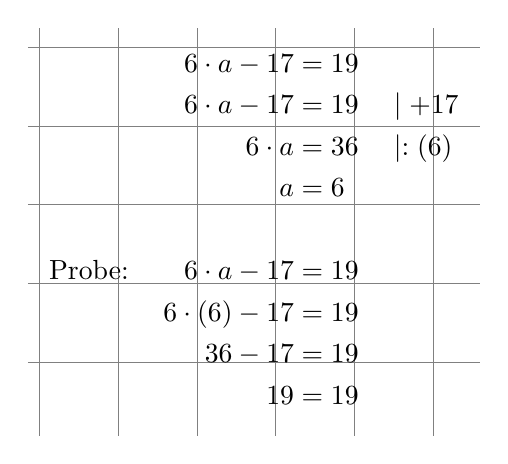
\begin{tikzpicture}[show background grid]
\node[below right] at (0,0.1) {
$\begin{aligned}
6\cdot a-17 &=19& &  \\
6\cdot a - 17 &=19& & \mid + 17\\
6\cdot a &=36& & \mid :\left(6\right)\\
a &=6& & 
\\
\\
\mbox{Probe:}\qquad 6\cdot a-17 &=19& &  \\
6\cdot \left(6\right)-17 &=19& &  \\
36-17 &=19& &  \\
19 &=19& &  \\
\end{aligned}$};
\end{tikzpicture}
\endgroup
&
f)&\begingroup\setlength{\jot}{-0.03cm}
\tikzstyle{background grid}=[draw, black!15,step=.5cm]
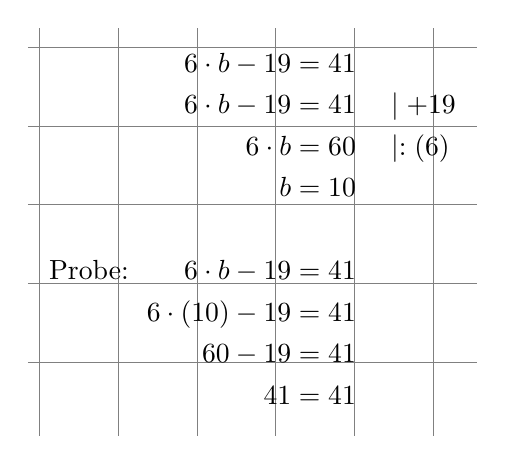
\begin{tikzpicture}[show background grid]
\node[below right] at (0,0.1) {
$\begin{aligned}
6\cdot b-19 &=41& &  \\
6\cdot b - 19 &=41& & \mid + 19\\
6\cdot b &=60& & \mid :\left(6\right)\\
b &=10& & 
\\
\\
\mbox{Probe:}\qquad 6\cdot b-19 &=41& &  \\
6\cdot \left(10\right)-19 &=41& &  \\
60-19 &=41& &  \\
41 &=41& &  \\
\end{aligned}$};
\end{tikzpicture}
\endgroup
\\\hline
g)&\begingroup\setlength{\jot}{-0.03cm}
\tikzstyle{background grid}=[draw, black!15,step=.5cm]
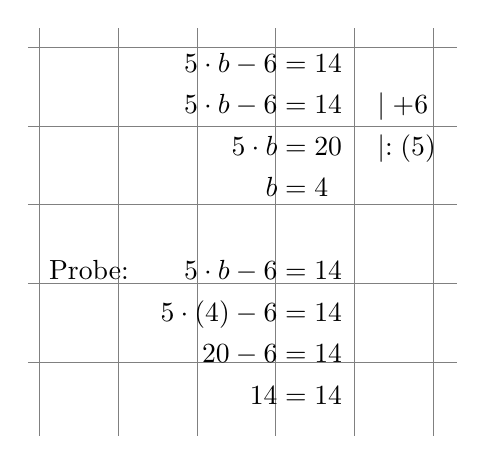
\begin{tikzpicture}[show background grid]
\node[below right] at (0,0.1) {
$\begin{aligned}
5\cdot b-6 &=14& &  \\
5\cdot b - 6 &=14& & \mid + 6\\
5\cdot b &=20& & \mid :\left(5\right)\\
b &=4& & 
\\
\\
\mbox{Probe:}\qquad 5\cdot b-6 &=14& &  \\
5\cdot \left(4\right)-6 &=14& &  \\
20-6 &=14& &  \\
14 &=14& &  \\
\end{aligned}$};
\end{tikzpicture}
\endgroup
&
h)&\begingroup\setlength{\jot}{-0.03cm}
\tikzstyle{background grid}=[draw, black!15,step=.5cm]
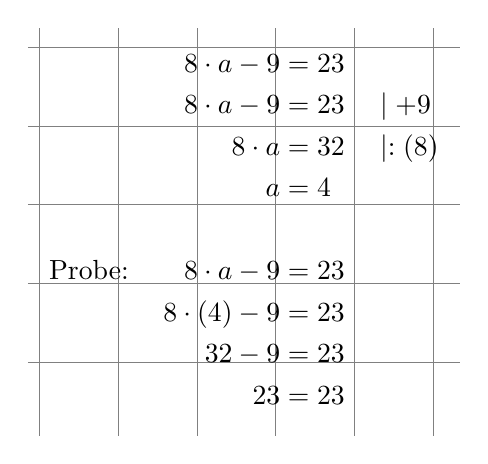
\begin{tikzpicture}[show background grid]
\node[below right] at (0,0.1) {
$\begin{aligned}
8\cdot a-9 &=23& &  \\
8\cdot a - 9 &=23& & \mid + 9\\
8\cdot a &=32& & \mid :\left(8\right)\\
a &=4& & 
\\
\\
\mbox{Probe:}\qquad 8\cdot a-9 &=23& &  \\
8\cdot \left(4\right)-9 &=23& &  \\
32-9 &=23& &  \\
23 &=23& &  \\
\end{aligned}$};
\end{tikzpicture}
\endgroup
\\\hline
i)&\begingroup\setlength{\jot}{-0.03cm}
\tikzstyle{background grid}=[draw, black!15,step=.5cm]
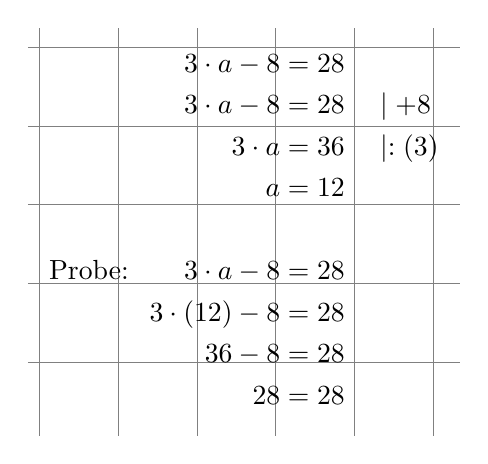
\begin{tikzpicture}[show background grid]
\node[below right] at (0,0.1) {
$\begin{aligned}
3\cdot a-8 &=28& &  \\
3\cdot a - 8 &=28& & \mid + 8\\
3\cdot a &=36& & \mid :\left(3\right)\\
a &=12& & 
\\
\\
\mbox{Probe:}\qquad 3\cdot a-8 &=28& &  \\
3\cdot \left(12\right)-8 &=28& &  \\
36-8 &=28& &  \\
28 &=28& &  \\
\end{aligned}$};
\end{tikzpicture}
\endgroup
&
j)&\begingroup\setlength{\jot}{-0.03cm}
\tikzstyle{background grid}=[draw, black!15,step=.5cm]
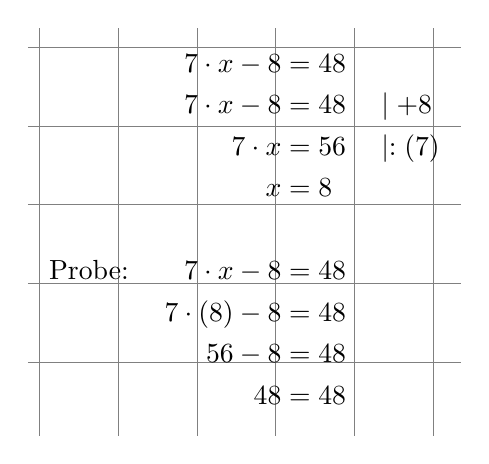
\begin{tikzpicture}[show background grid]
\node[below right] at (0,0.1) {
$\begin{aligned}
7\cdot x-8 &=48& &  \\
7\cdot x - 8 &=48& & \mid + 8\\
7\cdot x &=56& & \mid :\left(7\right)\\
x &=8& & 
\\
\\
\mbox{Probe:}\qquad 7\cdot x-8 &=48& &  \\
7\cdot \left(8\right)-8 &=48& &  \\
56-8 &=48& &  \\
48 &=48& &  \\
\end{aligned}$};
\end{tikzpicture}
\endgroup
\\\hline
k)&\begingroup\setlength{\jot}{-0.03cm}
\tikzstyle{background grid}=[draw, black!15,step=.5cm]
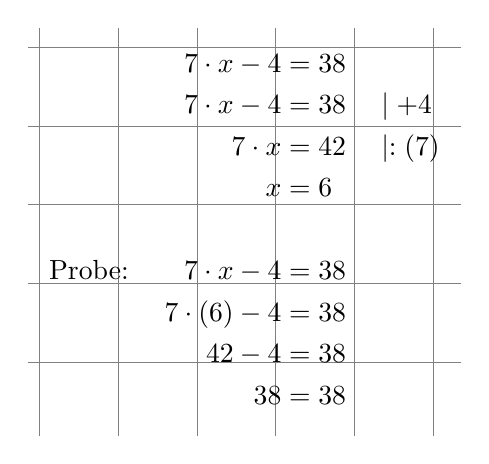
\begin{tikzpicture}[show background grid]
\node[below right] at (0,0.1) {
$\begin{aligned}
7\cdot x-4 &=38& &  \\
7\cdot x - 4 &=38& & \mid + 4\\
7\cdot x &=42& & \mid :\left(7\right)\\
x &=6& & 
\\
\\
\mbox{Probe:}\qquad 7\cdot x-4 &=38& &  \\
7\cdot \left(6\right)-4 &=38& &  \\
42-4 &=38& &  \\
38 &=38& &  \\
\end{aligned}$};
\end{tikzpicture}
\endgroup
&
l)&\begingroup\setlength{\jot}{-0.03cm}
\tikzstyle{background grid}=[draw, black!15,step=.5cm]
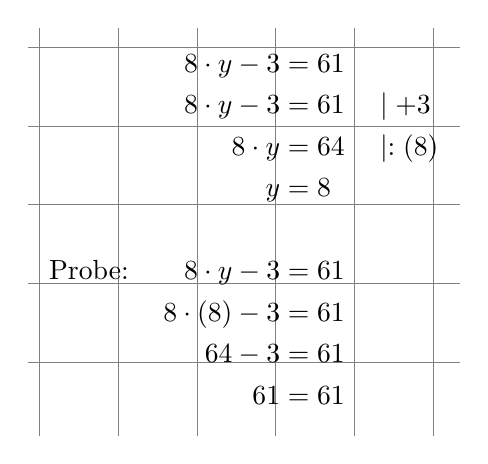
\begin{tikzpicture}[show background grid]
\node[below right] at (0,0.1) {
$\begin{aligned}
8\cdot y-3 &=61& &  \\
8\cdot y - 3 &=61& & \mid + 3\\
8\cdot y &=64& & \mid :\left(8\right)\\
y &=8& & 
\\
\\
\mbox{Probe:}\qquad 8\cdot y-3 &=61& &  \\
8\cdot \left(8\right)-3 &=61& &  \\
64-3 &=61& &  \\
61 &=61& &  \\
\end{aligned}$};
\end{tikzpicture}
\endgroup
\\\hline
m)&\begingroup\setlength{\jot}{-0.03cm}
\tikzstyle{background grid}=[draw, black!15,step=.5cm]
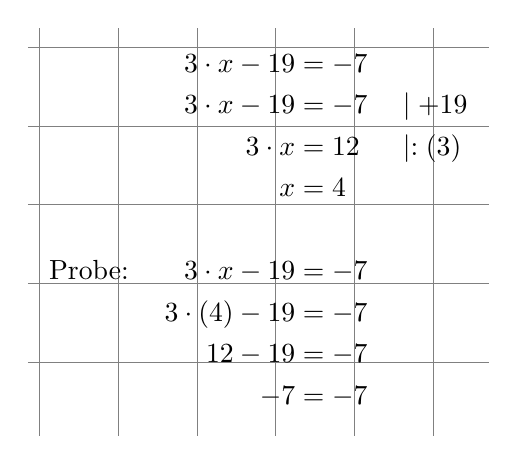
\begin{tikzpicture}[show background grid]
\node[below right] at (0,0.1) {
$\begin{aligned}
3\cdot x-19 &=-7& &  \\
3\cdot x - 19 &=-7& & \mid + 19\\
3\cdot x &=12& & \mid :\left(3\right)\\
x &=4& & 
\\
\\
\mbox{Probe:}\qquad 3\cdot x-19 &=-7& &  \\
3\cdot \left(4\right)-19 &=-7& &  \\
12-19 &=-7& &  \\
-7 &=-7& &  \\
\end{aligned}$};
\end{tikzpicture}
\endgroup
&
n)&\begingroup\setlength{\jot}{-0.03cm}
\tikzstyle{background grid}=[draw, black!15,step=.5cm]
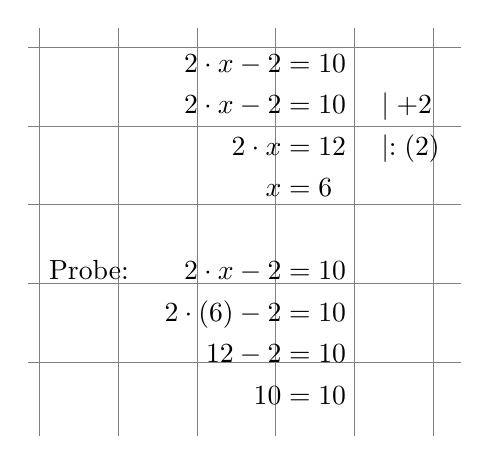
\begin{tikzpicture}[show background grid]
\node[below right] at (0,0.1) {
$\begin{aligned}
2\cdot x-2 &=10& &  \\
2\cdot x - 2 &=10& & \mid + 2\\
2\cdot x &=12& & \mid :\left(2\right)\\
x &=6& & 
\\
\\
\mbox{Probe:}\qquad 2\cdot x-2 &=10& &  \\
2\cdot \left(6\right)-2 &=10& &  \\
12-2 &=10& &  \\
10 &=10& &  \\
\end{aligned}$};
\end{tikzpicture}
\endgroup
\\\hline
o)&\begingroup\setlength{\jot}{-0.03cm}
\tikzstyle{background grid}=[draw, black!15,step=.5cm]
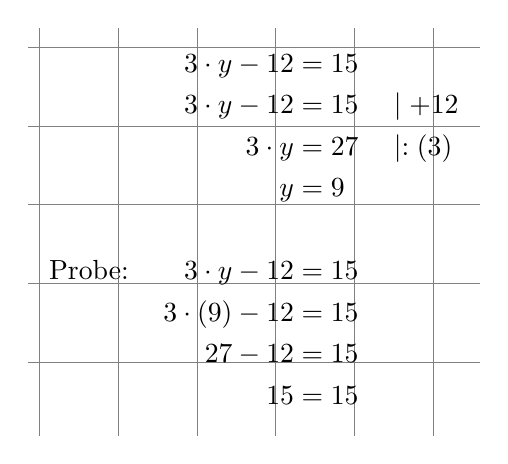
\begin{tikzpicture}[show background grid]
\node[below right] at (0,0.1) {
$\begin{aligned}
3\cdot y-12 &=15& &  \\
3\cdot y - 12 &=15& & \mid + 12\\
3\cdot y &=27& & \mid :\left(3\right)\\
y &=9& & 
\\
\\
\mbox{Probe:}\qquad 3\cdot y-12 &=15& &  \\
3\cdot \left(9\right)-12 &=15& &  \\
27-12 &=15& &  \\
15 &=15& &  \\
\end{aligned}$};
\end{tikzpicture}
\endgroup
&
p)&\begingroup\setlength{\jot}{-0.03cm}
\tikzstyle{background grid}=[draw, black!15,step=.5cm]
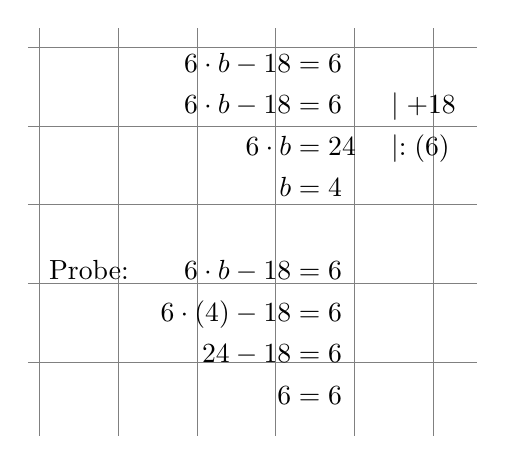
\begin{tikzpicture}[show background grid]
\node[below right] at (0,0.1) {
$\begin{aligned}
6\cdot b-18 &=6& &  \\
6\cdot b - 18 &=6& & \mid + 18\\
6\cdot b &=24& & \mid :\left(6\right)\\
b &=4& & 
\\
\\
\mbox{Probe:}\qquad 6\cdot b-18 &=6& &  \\
6\cdot \left(4\right)-18 &=6& &  \\
24-18 &=6& &  \\
6 &=6& &  \\
\end{aligned}$};
\end{tikzpicture}
\endgroup
\\\hline
q)&\begingroup\setlength{\jot}{-0.03cm}
\tikzstyle{background grid}=[draw, black!15,step=.5cm]
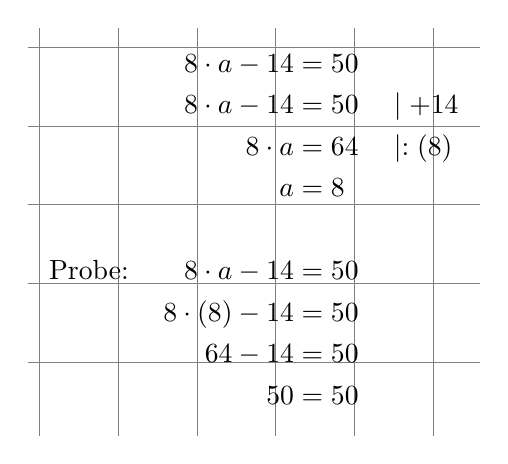
\begin{tikzpicture}[show background grid]
\node[below right] at (0,0.1) {
$\begin{aligned}
8\cdot a-14 &=50& &  \\
8\cdot a - 14 &=50& & \mid + 14\\
8\cdot a &=64& & \mid :\left(8\right)\\
a &=8& & 
\\
\\
\mbox{Probe:}\qquad 8\cdot a-14 &=50& &  \\
8\cdot \left(8\right)-14 &=50& &  \\
64-14 &=50& &  \\
50 &=50& &  \\
\end{aligned}$};
\end{tikzpicture}
\endgroup
&
r)&\begingroup\setlength{\jot}{-0.03cm}
\tikzstyle{background grid}=[draw, black!15,step=.5cm]
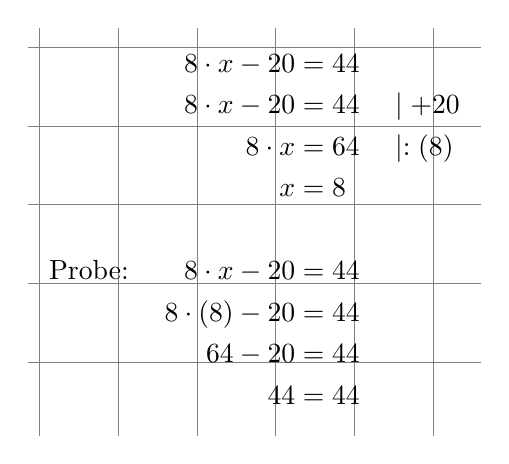
\begin{tikzpicture}[show background grid]
\node[below right] at (0,0.1) {
$\begin{aligned}
8\cdot x-20 &=44& &  \\
8\cdot x - 20 &=44& & \mid + 20\\
8\cdot x &=64& & \mid :\left(8\right)\\
x &=8& & 
\\
\\
\mbox{Probe:}\qquad 8\cdot x-20 &=44& &  \\
8\cdot \left(8\right)-20 &=44& &  \\
64-20 &=44& &  \\
44 &=44& &  \\
\end{aligned}$};
\end{tikzpicture}
\endgroup
\\\hline
s)&\begingroup\setlength{\jot}{-0.03cm}
\tikzstyle{background grid}=[draw, black!15,step=.5cm]
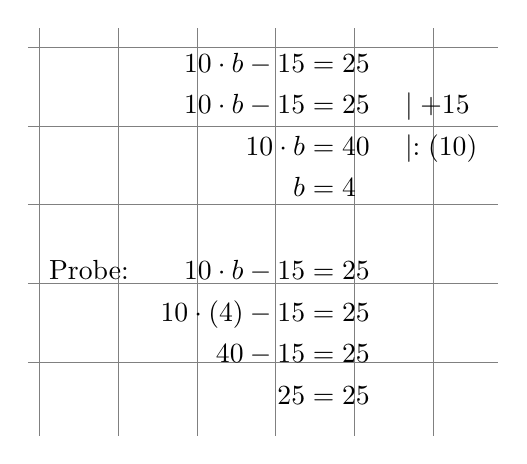
\begin{tikzpicture}[show background grid]
\node[below right] at (0,0.1) {
$\begin{aligned}
10\cdot b-15 &=25& &  \\
10\cdot b - 15 &=25& & \mid + 15\\
10\cdot b &=40& & \mid :\left(10\right)\\
b &=4& & 
\\
\\
\mbox{Probe:}\qquad 10\cdot b-15 &=25& &  \\
10\cdot \left(4\right)-15 &=25& &  \\
40-15 &=25& &  \\
25 &=25& &  \\
\end{aligned}$};
\end{tikzpicture}
\endgroup
&
t)&\begingroup\setlength{\jot}{-0.03cm}
\tikzstyle{background grid}=[draw, black!15,step=.5cm]
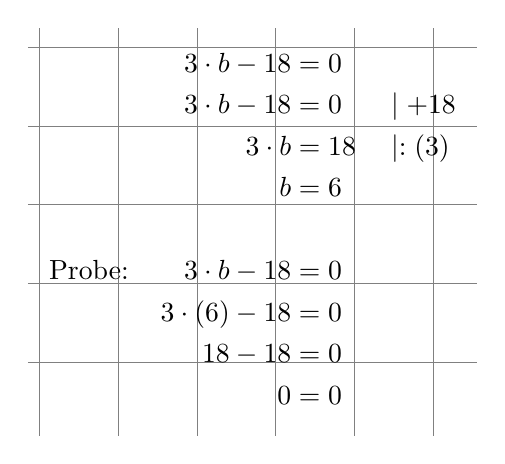
\begin{tikzpicture}[show background grid]
\node[below right] at (0,0.1) {
$\begin{aligned}
3\cdot b-18 &=0& &  \\
3\cdot b - 18 &=0& & \mid + 18\\
3\cdot b &=18& & \mid :\left(3\right)\\
b &=6& & 
\\
\\
\mbox{Probe:}\qquad 3\cdot b-18 &=0& &  \\
3\cdot \left(6\right)-18 &=0& &  \\
18-18 &=0& &  \\
0 &=0& &  \\
\end{aligned}$};
\end{tikzpicture}
\endgroup
\\\hline
u)&\begingroup\setlength{\jot}{-0.03cm}
\tikzstyle{background grid}=[draw, black!15,step=.5cm]
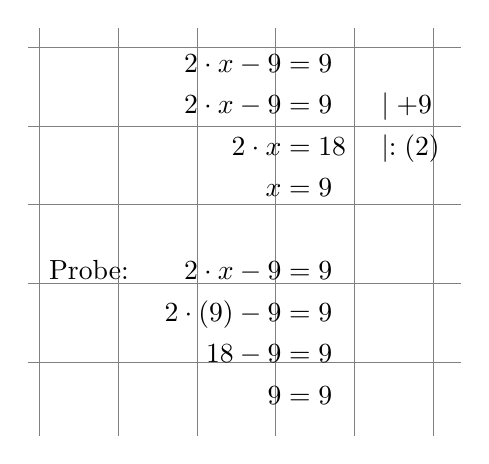
\begin{tikzpicture}[show background grid]
\node[below right] at (0,0.1) {
$\begin{aligned}
2\cdot x-9 &=9& &  \\
2\cdot x - 9 &=9& & \mid + 9\\
2\cdot x &=18& & \mid :\left(2\right)\\
x &=9& & 
\\
\\
\mbox{Probe:}\qquad 2\cdot x-9 &=9& &  \\
2\cdot \left(9\right)-9 &=9& &  \\
18-9 &=9& &  \\
9 &=9& &  \\
\end{aligned}$};
\end{tikzpicture}
\endgroup
&
v)&\begingroup\setlength{\jot}{-0.03cm}
\tikzstyle{background grid}=[draw, black!15,step=.5cm]
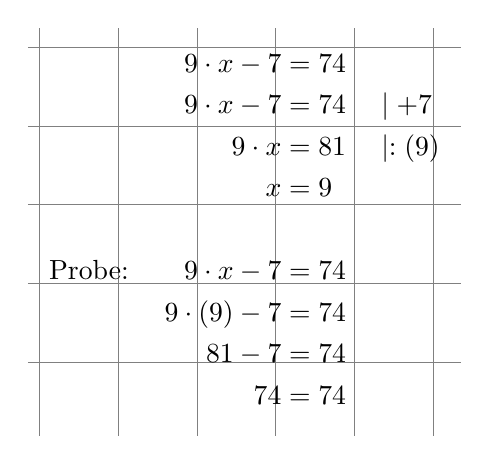
\begin{tikzpicture}[show background grid]
\node[below right] at (0,0.1) {
$\begin{aligned}
9\cdot x-7 &=74& &  \\
9\cdot x - 7 &=74& & \mid + 7\\
9\cdot x &=81& & \mid :\left(9\right)\\
x &=9& & 
\\
\\
\mbox{Probe:}\qquad 9\cdot x-7 &=74& &  \\
9\cdot \left(9\right)-7 &=74& &  \\
81-7 &=74& &  \\
74 &=74& &  \\
\end{aligned}$};
\end{tikzpicture}
\endgroup
\\\hline
w)&\begingroup\setlength{\jot}{-0.03cm}
\tikzstyle{background grid}=[draw, black!15,step=.5cm]
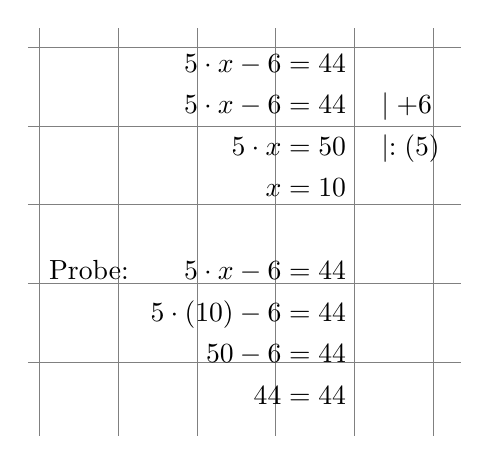
\begin{tikzpicture}[show background grid]
\node[below right] at (0,0.1) {
$\begin{aligned}
5\cdot x-6 &=44& &  \\
5\cdot x - 6 &=44& & \mid + 6\\
5\cdot x &=50& & \mid :\left(5\right)\\
x &=10& & 
\\
\\
\mbox{Probe:}\qquad 5\cdot x-6 &=44& &  \\
5\cdot \left(10\right)-6 &=44& &  \\
50-6 &=44& &  \\
44 &=44& &  \\
\end{aligned}$};
\end{tikzpicture}
\endgroup
&
x)&\begingroup\setlength{\jot}{-0.03cm}
\tikzstyle{background grid}=[draw, black!15,step=.5cm]
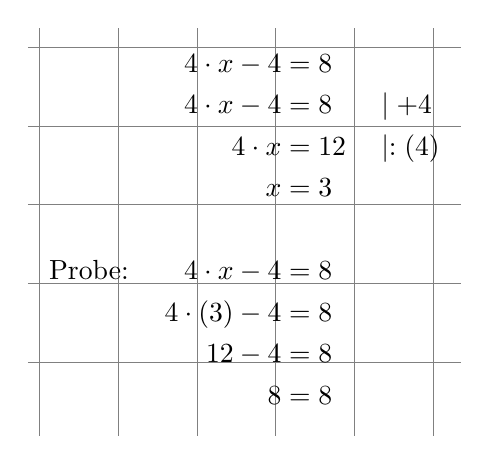
\begin{tikzpicture}[show background grid]
\node[below right] at (0,0.1) {
$\begin{aligned}
4\cdot x-4 &=8& &  \\
4\cdot x - 4 &=8& & \mid + 4\\
4\cdot x &=12& & \mid :\left(4\right)\\
x &=3& & 
\\
\\
\mbox{Probe:}\qquad 4\cdot x-4 &=8& &  \\
4\cdot \left(3\right)-4 &=8& &  \\
12-4 &=8& &  \\
8 &=8& &  \\
\end{aligned}$};
\end{tikzpicture}
\endgroup
\\\hline
y)&\begingroup\setlength{\jot}{-0.03cm}
\tikzstyle{background grid}=[draw, black!15,step=.5cm]
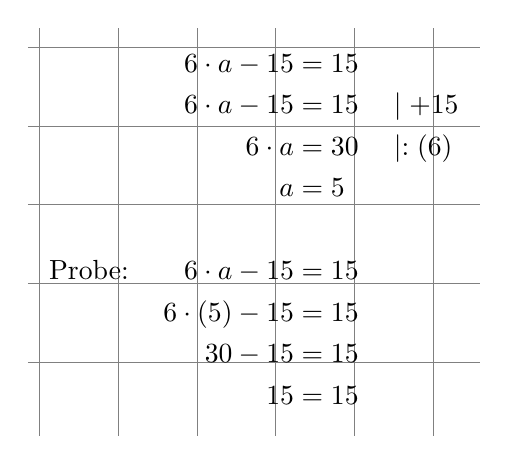
\begin{tikzpicture}[show background grid]
\node[below right] at (0,0.1) {
$\begin{aligned}
6\cdot a-15 &=15& &  \\
6\cdot a - 15 &=15& & \mid + 15\\
6\cdot a &=30& & \mid :\left(6\right)\\
a &=5& & 
\\
\\
\mbox{Probe:}\qquad 6\cdot a-15 &=15& &  \\
6\cdot \left(5\right)-15 &=15& &  \\
30-15 &=15& &  \\
15 &=15& &  \\
\end{aligned}$};
\end{tikzpicture}
\endgroup
&
z)&\begingroup\setlength{\jot}{-0.03cm}
\tikzstyle{background grid}=[draw, black!15,step=.5cm]
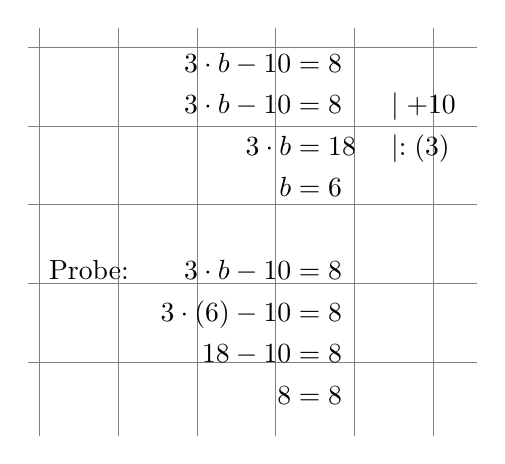
\begin{tikzpicture}[show background grid]
\node[below right] at (0,0.1) {
$\begin{aligned}
3\cdot b-10 &=8& &  \\
3\cdot b - 10 &=8& & \mid + 10\\
3\cdot b &=18& & \mid :\left(3\right)\\
b &=6& & 
\\
\\
\mbox{Probe:}\qquad 3\cdot b-10 &=8& &  \\
3\cdot \left(6\right)-10 &=8& &  \\
18-10 &=8& &  \\
8 &=8& &  \\
\end{aligned}$};
\end{tikzpicture}
\endgroup
\\\hline
\end{xltabular}
\vspace{0.5cm}
\end{document}